\documentclass[12pt]{report}

\usepackage[utf8]{inputenc}
\usepackage[T1]{fontenc}
\usepackage[magyar]{babel}

\usepackage{times}

\usepackage{amsmath}
\usepackage{amssymb}
\usepackage{amsthm}

\usepackage{fancyhdr}

\usepackage{graphicx}
\usepackage{psfrag}

\usepackage{listings}

\usepackage{url}

\usepackage{setspace}

\usepackage{enumitem}
\usepackage{todonotes}



%Margók:
\hoffset -1in
\voffset -1in
\oddsidemargin 35mm
\textwidth 150mm
\topmargin 15mm
\headheight 10mm
\headsep 5mm
\textheight 237mm

% Listing beállítások
\lstset{basicstyle=\small,  showstringspaces=false, breaklines=true}
\renewcommand{\lstlistingname}{Kódrészlet}

\definecolor{lightgray}{rgb}{.9,.9,.9}
\definecolor{darkgray}{rgb}{.4,.4,.4}
\definecolor{purple}{rgb}{0.65, 0.12, 0.82}

\lstdefinelanguage{typescript}{
  keywords={arguments,await,break,case,catch,class,const,continue,debugger,default,delete,do,else,enum,eval,export,extends,false,finally,for,function,if,implements,import,in,instanceof,interface,let,new,null,package,private,protected,public,return,static,super,switch,this,throw,true,try,typeof,var,void,while,with,yield}, % JavaScript ES6 keywords
  keywordstyle=\color{blue}\bfseries,
  ndkeywords={add, apply, args, Array, Array.from, Array.isArray, Array.of , Array.prototype, ArrayBuffer, bind, Boolean, call, charAt, charCodeAt, clear, codePointAt, concat, constructor, copyWithin, DataView, Date, Date.now, Date.parse, Date.prototype, Date.UTC, decodeURI, decodeURIComponent, encodeURI, encodeURIComponent, endsWith, entries, Error, Error.prototype, EvalError, every, false, fill, filter, find, findIndex, Float32Array, Float64Array, forEach, FulfillPromise, Function, Function.length, get, getDate, getDay, getFullYear, getHours, getMilliseconds, getMinutes, getMonth, getSeconds, getTime, getTimezoneOffset, getUTCDate, getUTCDay, getUTCFullYear, getUTCHours, getUTCMilliseconds, getUTCMinutes, getUTCMonth, getUTCSeconds, has,hasInstance, hasOwnProperty, ignoreCase, includes, indexOf, indexOf, Infinity, Int8Array, Int16Array, Int32Array, isConcatSpreadable, isFinite, isNaN, IsPromise, isPrototypeOf, Iterable, iterator, join, JSON, JSON.parse, JSON.stringify, keys, lastIndexOf, lastIndexOf, length, localeCompare, map, Map, match, match, Math, Math.abs , Math.acos, Math.acosh, Math.asin, Math.asinh, Math.atan, Math.atan2, Math.atanh, Math.cbrt, Math.ceil, Math.clz32, Math.cos, Math.cosh,  Math.E, Math.exp, Math.expm1, Math.floor, Math.fround, Math.hypot, Math.imul, Math.LN2, Math.LN10, Math.log, Math.log1p, Math.log2, Math.LOG2E, Math.log10, Math.LOG10E, Math.max, Math.min, Math.PI, Math.pow, Math.random, Math.round, Math.sign, Math.sin, Math.sinh, Math.sqrt, Math.SQRT1_2, Math.SQRT2, Math.tan, Math.tanh, Math.trunc, message, multiline, name, NaN, NewPromiseCapability, next, normalize, null, Number, Number.EPSILON, Number.isFinite, Number.isInteger, Number.isNaN, Number.isSafeInteger, Number.MAX_SAFE_INTEGER, Number.MAX_VALUE, Number.MIN_SAFE_INTEGER, Number.MIN_VALUE, Number.NaN, Number.NEGATIVE_INFINITY, Number.parseFloat, Number.parseInt, Number.POSITIVE_INFINITY, Number.prototype, Object, Object, Object.assign, Object.create, Object.defineProperties, Object.defineProperty, Object.freeze, Object.getOwnPropertyDescriptor, Object.getOwnPropertyNames, Object.getOwnPropertySymbols, Object.getPrototypeOf, Object.is, Object.isExtensible, Object.isFrozen, Object.isSealed, Object.keys, Object.preventExtensions, Object.prototype, Object.seal, Object.setPrototypeOf, of, parseFloat, parseInt, pop, Promise, Promise.all , Promise.race, Promise.reject, Promise.resolve, PromiseReactionJob, propertyIsEnumerable, prototype, Proxy, Proxy.revocable , push, RangeError, reduce, reduceRight, ReferenceError, Reflect, Reflect.apply, Reflect.construct , Reflect.defineProperty, Reflect.deleteProperty, Reflect.enumerate, Reflect.get, Reflect.getOwnPropertyDescriptor, Reflect.getPrototypeOf, Reflect.has, Reflect.isExtensible, Reflect.ownKeys, Reflect.preventExtensions, Reflect.set, Reflect.setPrototypeOf, Reflection, RegExp, RegExp, RegExp.prototype, repeat, replace, replace, reverse, search, search, Set, set, setDate, setFullYear, setHours, setMilliseconds, setMinutes, setMonth, setSeconds, setTime, setUTCDate, setUTCFullYear, setUTCHours, setUTCMilliseconds, setUTCMinutes, setUTCMonth, setUTCSeconds, shift, slice, slice, some, sort, species, splice, split, split, startsWith, String, String.fromCharCode, String.fromCodePoint, String.raw, substring, Symbol, Symbol.for, Symbol.hasInstance, Symbol.isConcatSpreadable, Symbol.iterator, Symbol.keyFor, Symbol.match, Symbol.prototype, Symbol.replace, Symbol.replace, Symbol.search, Symbol.species, Symbol.split, Symbol.toPrimitive, Symbol.toStringTag, Symbol.unscopables, SyntaxError, then, toDateString, toExponential, toFixed, toISOString, toJSON, toLocaleDateString, toLocaleLowerCase, toLocaleString, toLocaleString, toLocaleString, toLocaleString, toLocaleTimeString, toLocaleUpperCase, toLowerCase, toPrecision, toPrimitive, toString, toStringTag, toTimeString, toUpperCase, toUTCString, TriggerPromiseReactions, trim, true, TypeError, Uint8Array, Uint8ClampedArray, Uint16Array, Uint32Array, undefined, unscopables, unshift, URIError, valueOf, WeakMap, WeakSet},
  ndkeywordstyle=\color{darkgray}\bfseries,
  identifierstyle=\color{black},
  sensitive=false,
  comment=[l]{//},
  morecomment=[s]{/*}{*/},
  commentstyle=\color{purple}\ttfamily,
  stringstyle=\color{red}\ttfamily,
  morestring=[b]',
  morestring=[b]"
}

\lstset{
   language=typescript,
   backgroundcolor=\color{lightgray},
   extendedchars=true,
   basicstyle=\footnotesize\ttfamily,
   showstringspaces=false,
   showspaces=false,
   numbers=left,
   numberstyle=\footnotesize,
   numbersep=9pt,
   tabsize=2,
   breaklines=true,
   showtabs=false,
   captionpos=b
}



\begin{document}

%A FEJEZETEK KEZDÕOLDALAINAK FEJ ES LÁBLÉCE:
%a plain oldalstílust kell átdefiniálni, hogy ott ne legyen fejléc:
\fancypagestyle{plain}{%
%ez mindent töröl:
\fancyhf{}
% a láblécbe jobboldalra kerüljön az oldalszám:
\fancyfoot[R]{\thepage}
%elválasztó vonal sem kell:
\renewcommand{\headrulewidth}{0pt}
}

%A TÖBBI OLDAL FEJ ÉS LÁBLÉCE:
\pagestyle{fancy}
\fancyhf{}
\fancyhead[L]{Fraktál bemutató keretrendszer}
\fancyfoot[R]{\thepage}


%A címoldalra se fej- se lábléc nem kell:
\thispagestyle{empty}

\begin{center}
\vspace*{1cm}
{\Large\bf Szegedi Tudományegyetem}

\vspace{0.5cm}

{\Large\bf Informatikai Intézet}

\vspace*{3.8cm}


{\LARGE\bf Fraktál bemutató keretrendszer }


\vspace*{3.6cm}

{\Large Szakdolgozat}

\vspace*{4cm}

%Értelemszerûen megváltoztatandó:
{\large
\begin{tabular}{c@{\hspace{4cm}}c}
\emph{Készítette:}     &\emph{Témavezetõ:}\\
\bf{Péter Albert}  &\bf{Tóth Zotán Gábor}\\
programtervező informatikus     &egyetemi tanársegéd\\
szakos hallgató&
\end{tabular}
}

\vspace*{2.3cm}

{\Large
Szeged
\\
\vspace{2mm}
\the\year
}
\end{center}


%A tartalomjegyzék:
\tableofcontents


\chapter*{Feladatkiírás}
%A tartalomjegyzékben mégis szerepeltetni kell, mint szakasz(section) szerepeljen:
\addcontentsline{toc}{section}{Feladatkiírás}
\spacing{1.5}
A szakdolgozatom központi témájául a fraktálokat választottam. Matematikában nem túl jártas egyéneknek lehetséges, hogy nem túl sokat mondó az a fogalom, hogy fraktál. Az én célom egy olyan webes applikáció elkészítése volt, amelyet használva mindenki mélyebb belátást nyerhet a fraktálok világába. A webes applikációban nyolc előre megírt algoritmus szerint generálhatunk fraktálokat. A felhasználóknak lehetőségük van az algoritmusok testreszabására, minden algoritmus egyéni konfigurálási lehetőségekkel rendelkezik. Ilyenek például az elforgatási szög módosítása, tetszőleges méretű, pozíciójú, valamint tetszőlegesen rotálható gyökér elem megadása, növekedés irányának módosítása, szín beállítása... Az applikáció arra is lehetőséget biztosít, hogy valamely időpontban az algoritmus futását szüneteljük, valamint ha szeretnénk, egy csúszka használatával visszatekerhetjük az algoritmus pillanatnyi állapotát valamely előző állapotra. Ezen kívül az alkalmazásban egy olyan funkció is található, amely segítségével a felhasználók a fraktálok generálása az adott fraktálról egy rövid leírást olvashatnak, ezzel is lehetőséget adva a felhasználóknak, hogy tudásukat bővítsék. Végül a generált fraktálokat kép formájában kiexportálhatjuk a saját gépünkre, ha szeretnénk.


\chapter*{Tartalmi összefoglaló}
\addcontentsline{toc}{section}{Tartalmi összefoglaló}
\spacing{1.5}
A dolgozat legfőbb célja a webalkalmazás működésének és fejlesztési menetének bemutatása. A feladat egy fraktál bemutató keretrendszer elkészítése volt, amelyben többek között olyan hasznos funkciók találhatók, mint az algoritmusok konfigurálhatósága, az algoritmusok futásának szüneteltetése, az algoritmusok állapotának visszaállítása egy korábbi állapotra, illetve a generált fraktál kiexportálása kép formájában. A dolgozat magába foglal egy bevezető szekciót, ahol a fraktálokról általános tudnivalókat olvashatunk. Itt lényegében a fraktálok eredetéről, fontosabb tulajdonságairól, illetve főbb felhasználási területeiről van szó. Ezen kívül, a dolgozat további részeiben magáról a webalkalmazásról van szó, ismertetem a felhasznált technológiákat, valamint részletezem a fejlesztés menetét.
\chapter{Bevezetés}
%\addcontentsline{toc}{section}{Bevezetés}
\spacing{1.5}

\section{A fraktálokról átalánosságban}
A fraktálok egy viszonylag újnak nevezhető terület a matematikában, és habár komolyabban vizsgálni őket csak a számítógépek megjelenése után kezdték el igazán, már a XX. század előtt is foglalkoztak a matematikusok ezekkel a különös geometriai alakzatokkal. Az elnevezést 1975-ben Benoît Mandelbrot adta, a latin fractus (vagyis törött, törés) szó alapján, ami az ilyen alakzatok tört számú dimenziójára utal, bár nem minden fraktál tört dimenziós (ilyenek például a síkkitöltő görbék)~\cite{fraktal} . 
Tört dimenziósnak nevezik azokat az alakzatokat, amelyek nincs területük, többek mint egy egyenes, viszont kevesebbek mint egy síkidom. Nagyszerű példa erre a Sierpiński-szőnyeg. Mandelbrot {\it The Fractal Geometry of Nature (A Természet Fraktálgeometriája)} című munkája mutatta be, és magyarázta el először a fogalmakat, melyek alapjául szolgálnak ennek az új területnek~\cite{fraktal-wiki}. 
\par A fraktálok önhasonló, végtelenül komplex matematikai alakzatok, melyek változatos formáiban legalább egy felismerhető ismétlődés tapasztalható. Az önhasonlóság azt jelenti, hogy egy kisebb rész felnagyítva ugyanolyan struktúrát mutat, mint egy nagyobb rész. Ilyen bizonyos léptékig például a természetben a villám mintázata, a levél erezete, a hópelyhek alakja, a fa ágai. A fraktál szóval rendszerint az önhasonló alakzatok közül azokra utalnak, amelyeket egy matematikai formulával le lehet írni, vagy meg lehet alkotni~\cite{fraktal}. A fraktálok egy másik tulajdonsága, hogy sehol sem differenciálhatók. Ennek oka az, hogy bár a fraktálok folytonosak, végtelenül gyűröttek. A fraktálokat úgy írhatjuk le, hogy megvizsgáljuk, hogyan változnak különböző felbontásoknál.

\section{A fraktálok felhasználási területei}
A fraktálok gyakorlati felhasználásának köre folyamatosan bővül. Rengeteg helyen találkozhatunk velük a művészetektől az orvosláson át a számítástechnikáig. Ma már bizonyított tény, hogy fraktálok, illetve fraktálszerű alakzatok a természetben is gyakran előfordulnak. Megfigyelések alapján tudjuk, hogy ezek az alakzatok egy meghatározott növekedési struktúrát követnek. Ilyenek a fák, kristályok, vagy a felhők. Számtalan művész használta a fraktálok ábrázolásának technikáját, annak ellenére, hogy pontos definícióját, matematikai hátterét nem ismerték.
Olyan neveket érdemes itt megemlíteni, mint például Vincent Van Gogh, vagy akár Maurits Cornelis Escher. A építészetben is sok önismétlődő részletet találhatunk gondoljunk csak a gótikus és barokk épületek ismétlődő támpilléreire, oszlopsoraira~\cite{alkalmazas}.
\par A fraktálok kiválóan alkalmazhatóak képi és hanganyag tömörítésére, feldolgozására. Ha egy hangot vagy képet fraktálokra bontunk, utána az adott darabot leíró algoritmussal és paramétereivel könnyen összehasonlíthatóvá válnak. Továbbá az algoritmusok és a hozzá tartozó paraméterek letárolása kevesebb területet vesz igénybe, mintha a nyers adatokat tárolnánk le~\cite{alkalmazas}.
\chapter{Háttér}
\spacing{1.5}

Az alkalmazás elkészítése előtt kiválasztottam azokat a fraktálgeneráló algoritmusokat, amelyeket implementálni szerettem volna. Nyolc algoritmus mellett döntöttem, ezek a következők: 
\begin{itemize}
	\item Sierpiński- háromszög
	\item Sierpiński-szőnyeg
	\item Fraktál-fa
	\item Pitagorasz-fa
	\item Lévy C-görbe
	\item Koch-görbe
	\item Hilbert-görbe
	\item H-fa
\end{itemize}
Választáskor többek között figyelembe vettem az algoritmusok bonyolultságát, milyen, és mennyi konfigurációs lehetőséggel tudom felruházni őket, valamint a fraktálok fajtáját. A választott algoritmusok között vannak helykitöltő algoritmusok is, mint például a Hilbert-görbe és a H-fa. Ezek az algoritmusok nagyjából kivétel nélkül már mások által implementálva vannak, a forráskódjuk bárki számára elérhető az interneten, viszont ezek az implementációk egyike sem támogatja a konfigurálhatóságot, ami az én alkalmazásom egyik alapköve. 
\par Mielőtt az implementációnak nekikezdtem, utánanéztem olyan webes alkalmazásoknak, amik hasonlóak, mint amit én is szerettem volna megvalósítani. Találtam hasonlót, ahol némelyik fraktálgeneráló algoritmus valamilyen szinten konfigurálható, viszont ezek az alkalmazások jellemzően csak egy-egy fraktállal foglalkoznak különösebben, így csak az adott fraktál generálására van lehetőségünk, valamint kevesebb konfigurálási lehetőséggel rendelkeznek, mint az én tervezett webalkalmazásom. Ezen kívül nem támogatnak kiexportálási és visszatekerési funkciókat. Az algoritmusok konfigurálása ezekben az alkalmazásokban egyszerű, jelölőnégyzettel, vagy számok bevitelére alkalmas mezőkkel történik, hasonlóan, mint ahogyan én is terveztem. 
\par Az interneten való keresgélést követően kiválasztottam azt a technológiát, amellyel magát a keretrendszert szerettem volna implementálni.
Mivel ez egy webes alkalmazás, a választás az Angular keretrendszerre esett, pontosabban annak a 8-as verziójára~\cite{angular}. Ez nem a legfrissebb verziója az Angular keretrendszernek, viszont korábban is használtam, és stabilitás szempontjából ez az egyik legjobb, ugyanis vannak olyan különböző API-k, amelyek még nem teljesen kompatibilisek az Angular legújabb verziójával. A fontosabb Angular API-k, amiket használtam a fejlesztés során a következők: Angular Material, Angular Flex Layout és Rxjs. Az Angular egy TypeScript keretrendszer, amellyel, a benne található csomagok segítségével rendkívül kényelmesen és könnyen készíthetünk Single Page webalkalmazásokat. Ezen kívül a JavaScript-es könyvtárak nagy részével kompatibilis, ami nagyon előnyös volt számomra, hiszen az algoritmusokat P5.js-ben implementáltam, ami egy nyílt forráskódú, vászon alapú rajzolásra alkalmas JavaScript könyvtár~\cite{p5}. Az alapok nagyon könnyen elsajátíthatóak, és a közismert alakzatok nagy részének rajzolása előre megírt függvények segítségével történik, ami rendkívül kényelmessé teszi a használatát. Ezen kívül vektorok használatát is támogatja, a vektorműveletek már előre definiálva vannak benne, amelyeket az algoritmusok implementálásakor előszeretettel használtam. Egyik funkcionalitása, ami még nagyon sokat segített az algoritmusok implementálásakor, az a $translate$ függvény, amely segítségével a vászon koordinátarendszerének origóját tudjuk eltolni. Ez egy rendkívül hasznos metódus, különböző rotációknál, és olyan alakzatok rajzolásánál, amelyek pozíciója az egérmutató elhelyezkedésétől függ. Ezek a műveletek az előre megírt függvényeknek köszönhetően sokkal kevesebb számolással kivitelezhetőek.
\par
A fejlesztés Windows 10 operációs rendszer alatt történt. A programozáshoz, futtatáshoz, teszteléshez a Visual Studio Code fejlesztői környezetet használtam. A szoftver verziókövetése, illetve a fájlok tárolása GitHub repository-n keresztül valósult meg.

\chapter*{Az alkalmazás alapfunkciói}
\addcontentsline{toc}{section}{Az alkalmazás alapfunkciói}
\spacing{1.5}
A alábbi fejezetben az elkészült alkalmazás főbb funkcióit mutatom be, fejtem ki részletesen, külön kitérve a fontosabb, érdekesebb részekre.
\section*{Lejátszást vezérlő funkciók}
A fraktál generáló algoritmusok futását három gombbal tudjuk vezérelni, ezek a Play, Pause és Start gombok. Mivel az alkalmazást megpróbáltam minél több komponensre bontani, így kellett egy külön szolgáltatás, amelynek a feladata az volt, hogy az egyes eseményeket, amelyeket a felhasználók a gombok megnyomásával váltanak ki, közvetítse az algoritmusnak, amely a fraktál generálására szolgál. Így az algoritmus tudni fogja mikor kell szünetelni, mikor kell rajzolni, és mikor kell újrakezdeni. A szolgáltatás kódja a következőképpen néz ki:
\begin{lstlisting}[language=typescript]
export class AnimationStateManagerService {
	private state: BehaviorSubject<boolean>;

	constructor() {
		this.state = new BehaviorSubject<boolean>(false);
	}
	
	setState(state: boolean): void {
		this.state.next(state);
	}
	
	getState(): Observable<boolean> {
		return this.state;
	}
}
\end{lstlisting}
A szolgáltatás alapja tehát egy {\it BehaviorSubject} objektum, amely {\it boolean} típusú adatot tud közvetíteni a feliratkozóknak. Amikor a felhasználó a lejátszást vezérlő gombok egyikével interakcióba lép, a szolgálatás {\it setState()} metódusa hívódik meg, amelynek a paramétere egy igaz-hamis adat, attól függően, hogy az algoritmus futása szünetel-e vagy sem. Amikor ez a metódus meghívódik, akkor a szolgáltatás a paraméterként kapott változó értéket közvetíti a feliratkozóknak, így azok tudni fogják, hogy a felhasználó interakcióba lépett a vezérlő gombok valamelyikével. A feliratkozó ebben az esetben az algoritmus, amely az adott fraktált generálja.  
\section*{Algoritmus lista és konfigurációs panelek}
A webalkalmazás két oldalsó panellel rendelkezik. Bal oldalon a fraktál generáló algoritmusok egy oszlopba rendezett listáját tekinthetjük meg. Az algoritmusok mindegyike rendelkezik előnézettel, tehát aki nem ismerné valamelyik algoritmust, láthatja, hogy az adott algoritmus milyen fraktált generál. Ezek az előnézetek maguknak az algoritmusoknak egy lebutított változatai, konfigurációs lehetőségek nélkül, az adott algoritmusok paraméterei alapértékekre vannak állítva. Minden algoritmus előnézete egy bizonyos szintig iterál, majd ha ezt a szintet elérte, újraindul. 
\par Jobb oldalon a konfigurációs panel található. Ennek a tartalma dinamikus, aszerint generálódik, hogy az adott algoritmusnak milyen konfigurációs lehetőségei vannak. A konfigurálás három féle módon történhet:
\begin{itemize}
	\item  csúszka segítségével állíthatunk be értéket az adott algoritmus valamely paraméterének, egy megadott értékkészleten belül
	\item jelölőnégyzet ki-be pipálásával tudjuk jelezni, hogy az adott konfigurációs lehetőséget használni szeretnénk-e
	\item színpaletta segítségével tudjuk a fraktál színét beállítani
\end{itemize}
\par Az algoritmusok listáját egy külön szolgáltatás tárolja. Minden komponens, amelynek szüksége van erre a listára, mint például a fent említett két panel, ettől a szolgáltatástól kéri el. Az algoritmusok listájának modellje a következőképpen néz ki:
\begin{lstlisting}[language=typescript]
export interface IAlgorithmList {
	name: string;
	previewId: string;
	preview: any;
	algorithm: any;
	configurations: IAlgorithmConfiguration[];
	about: string;
}
\end{lstlisting}
Az algoritmusok listájában tárolódik tehát minden algoritmus
\begin{itemize}
	\item neve
	\item előnézetének azonosítója, amely az előnézet megjelenítéséhez kell
	\item a fraktál előnézetét kirajzoló algoritmus referenciája, amely a tényleges algoritmus egy lebutított változata
	\item a tényleges algoritmus referenciája, amely már konfigurációs lehetőségekkel rendelkezik
	\item az adott algoritmus konfigurációs lehetőségei, tömbben tárolva
	\item egy pár mondatos ismertető az adott algoritmusról, ez egy külön funkció lételeme, amelyről a későbbiekben lesz szó
\end{itemize}
A lista panelnek az algoritmusok előnézet azonosítójára, és az előnézet algoritmus referenciájára van szüksége, a konfigurációs panelnek pedig az algoritmusok konfigurációs lehetőségeire, amelyek tömbben tárolódnak. Ezen kívül mindkét panel eltüntethető és előhozható egy-egy gomb segítségével, ezzel is növelve az alkalmazás kompaktságát. Az eltüntetés és előhozás animációval történik, amely abból áll, hogy gomb megnyomásra, CSS szinten tolom a panelek pozicíóját X tengelyen jobb vagy balra, attól függően, hogy előhozni, vagy eltüntetni szeretnénk a paneleket. Az animáció megvalósítására az Angular Animations API-ját használtam. Ennek a menete, hogy a CSS animációkat egy tömbben definiáltam, majd hozzákötöttem az adott panelekhez egy boolean változó segítségével. A boolean változó értéke a gomb nyomására változik, így fogja tudni az alkalmazás, hogy eltüntetni, vagy megjeleníteni kell.

\section*{Visszatekerés funkció}
A visszatekerés funkció egy sajátos funkciója az alkalmazásomnak, hiszen egy hasonló alkalmazás sem rendelkezik ilyen lehetőséggel. Alapja egy csúszka, ami, ha a felhasználó interakcióba lép vele, az algoritmust visszatekerő módba helyezi. A csúszka kódja az alábbi módon néz ki:
\begin{lstlisting}[language=html]
<div class="slider-container">
<input #slider (click)="rollBack(slider.value)" type="range" min="0" [max]="sliderLength" [value]="sliderLength" class="slider" id="myRange">
</div>
\end{lstlisting}
Lényegében ez egy egyéni stílusú, range típusú input mező, amelynek a max és a value direktivákkal lehet értéket beállítani. A value paraméter mondja meg, hogy a csúszka éppen hol áll, ez alapértelmezetten 0-ra van állítva. A max paraméter azt adja meg, hogy a csúszka milyen hosszúságú, ennek az értéke az algoritmus futásával párhuzamosan változik, amit egy BehaviourSubject típusú változóval oldottam meg. Lényegében, amikor az algoritmus egy új iterációját rajzolja le a fraktálnak, ez a BehaviorSubject objektum egy új értéket közvetít a feliratkozóknak, aki jelen esetben a csúszka, így annak a hossza mindig a megfelelő értékre lesz beállítva. Ha a csúszkára kattint a felhasználó, az adott algoritmus visszatekerő módba kerül, és meghívódik a rollBack metódusa, amellyel minden algoritmus rendelkezik. A visszatekeró mód annyit jelent, hogy beállítódnak azok az értékek, amelyeket kiolvasva, az algoritmus tudni fogja meddig kell visszatekerni a fraktált. Ennek a kódja így néz ki:
\begin{lstlisting}
rollBack(p: any) {
	if (this.rollBack) {
		if (this.play) {
			for (let i = 0; i < this.list.length; i++) {
				this.list[i].draw(p);
			}
			this.rollBack = false;
		}
		else {
			p.background(this.canvasColor);
			for (let i = 0; i < this.rollBackTo; i++) {
				this.list[i].draw(p);
			}
		}
	}
}
\end{lstlisting}
Ez a függvény minden képfrissítéskor újrarajzolja a hátteret, ennek köszönhetően eddig megrajzolt alakzat törlődik a vászonról. Ezután a függvény végigiterál azon a listán, amelyben az algoritmus tárolja a visszatekerés előtt még megrajzolt alakzatokat, és ez alapján rajzolja vissza azokat az elemeket, amelyek szükségesek. Minden algoritmus rendelkezik ilyen listával, hiszen ez a visszatekerés funkciójának egy fontos alapeleme.
\section*{Fraktál leírás funkció}
Mindegyik fraktált generáló algoritmus rendelkezik egy leírással. Ebben a leírásban egy rövid ismeretőt olvashatunk az adott fraktálról, ki fedezte fel, hol használják, jellegzetes tulajdonságok megemlítése. A leírást egy előugró ablak tartalmazza. Ez az előugró ablak egy globális komponens, minden algoritmus esetén ugyanaz az ablak ugrik elő, csupán a tartalma változik dinamikusan. Az ablakot egy gomb megnyomásával hívhatjuk elő. Az ablak HTML kódja így néz ki:
\begin{lstlisting}[language=html]
<div>
	<h1>{{data.title}}</h1>
	<p>{{data.about}}</p>
	<button (click)="close()" mat-button>Bezar</button>
</div>
\end{lstlisting}
Ez egy eléggé rövid kódsor, azonban látszik, hogy a címet és magát a leírást a data változó tartalmazza. A data változó akkor definiálódik, amikor az ablakot előhozó gombra kattint a felhasználó, az értéke pedig az algoritmus listából olvasódik ki, attól függően, hogy éppen melyik fraktál generáló algoritmus aktív. A gomb megnyomására a következő függvény fut le:
\begin{lstlisting}[language=typescript]
about(): void {
	let dialogRef = this.dialog.open(AboutComponent, {
		width: '800px',
		data: {
			title: this.title,
			about: this.algorithmList[this.activeAlgorithm].about
		}
	});
}
\end{lstlisting}
A width property értelemszerűen az előugró ablak szélességét adja meg, ebben az esetben az ablak 800 pixel széles lesz. Magasságot azért nem definiáltam, hogy különböző hosszúságú szövegek esetén se csússzon szét az ablak, a data változóról pedig pár sorral fentebb volt szó.
\chapter*{Algoritmusok}
\addcontentsline{toc}{section}{Algoritmusok}
\spacing{1.5}
Ebben a fejezetben azokról az fraktál generáló algoritmusokról lesz szó, amelyeket a webalkalmazás részeként leimplementáltam. Minden algoritmusról egy először rövid ismertetőt írok, majd bemutatom az implementáció menetét. Azonban még mielőtt ebbe belekezdenék, szeretnék egy pár fogalmat tisztázni.
\par A Hausdorff-dimenzió a fraktáloknál használt dimenziófogalom, melynek bevezetését az indokolja, hogy egyes alakzatok, ide tartozik a fraktálok sokasága, kerülete, területe, és egyéb dimenzióbeli mértékei ellentmondásos értéket adnak. Például a Sierpiński-szőnyeg lefed egy négyzetet, tehát kétdimenziós, viszont a hézagoknak köszönhetően a területe 0, akárcsak az egydimenziós alakzatoké. A szokásos alakzatok körében a Hausdorff-dimenzió megegyezik az ismert értékekkel: az egyenesé 1, a négyzeté 2, a kockáé 3. Ez abból fakad, hogy a Haussdorff-dimenzió a hosszúság és a terület mérésén alapul. A Hausdorff-dimenzió tehát, a hagyományos, pozitív egész számokkal mérhető dimenziófogalom általánosítása. A Hausdorff-dimenzió nem feltétlenül egész szám.
\par Amit még szeretnék egy pár mondatban megfogalmazni az a p5.js könyvtár működési elve. A p5.js-ben történő rajzoláshoz két függvényt kell megvalósítani. Ezek a setup és a draw függvények. A setup függvény a rajzolás elkezdése előtt fut le egyszer, ez tipikusan a vászon létrehozására, háttér, szín, képfrissítés, és egyéb tulajdonságok beállítására használatos. Maga a rajzolás a draw függvényben történik. Ez a függvény minden másodpercben annyiszor fut le amennyi a képfrissítés tulajdonság értéke, ez alapértelmezetten 60-ra van állítva a legtöbb számítógép esetében. 
\section*{Sierpiński-háromszög}
A Wacław Sierpiński lengyel matematikus által megtalált fraktál úgy áll elő, hogy egy szabályos háromszögből elhagyjuk az oldalfelező pontok összekötésével nyert belső háromszöget, majd az így maradt három háromszögre rekurzívan alkalmazzuk ugyanezt az eljárást.
A Sierpiński-háromszög konstrukciójához többnyire egyenlő oldalú háromszöget választanak. Ez azonban nem kötelező, bármely háromszögből lehet Sierpiński-háromszöget készíteni.
Az általam megírt algoritmus az alábbi lépések szerint generálja ezt a fraktált:
\begin{itemize}
\item Vegyünk három pontot, melyek a háromszöget határolják be, mindegyik pont a háromszög egy csúcsa
\item Rajzoljunk egy pontot egy tetszőleges helyre, ez lesz a kezdőpont
\item Válasszuk ki a háromszög egyik csúcsát valamilyen véletlenszerű módon, majd a választott csúcsot és a kezdőpontot összekötő képzeletbeli vonal közepére rajzoljunk be egy újabb pontot, ez lesz az új kezdőpont
\item Ismételjük meg ezeket a lépéseket
\end{itemize}
\begin{figure}[!ht]
\begin{center}
	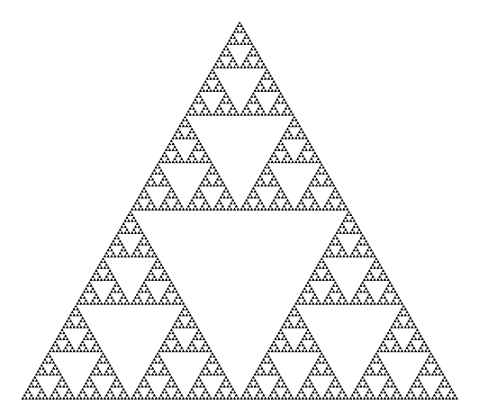
\includegraphics[width=0.5\textwidth]{img/SierpinskiTriangle}
	\caption[labelInTOC]{Sierpiński-háromszög}
\end{center}
\end{figure}
Minden lépésben a keletkező kis háromszögek oldalhossza megfeleződik, és területük a negyedére csökken, miközben a középső háromszög eltűnik.\\
A Sierpiński háromszög Hausdorff-dimenziója: $log(3)/log(2) = 1,585$
\subsection*{Implementáció}
A Sierpiński-háromszög implementációjának kezdéseként először egy segédosztályt írtam, mint ahogy a többi algoritmus nagy részének implementációja is segédosztályok segítségével valósult meg. Ez a segédosztály a Point osztály, mivel a Sierpiński-háromszöget az algoritmus pontok segítségével rajzolja ki. Itt definiálva vannak a pontokhoz tartozó adattagok, ez ebben az esetben egy vektor, ami tárolja egy adott pont x és y pozícióját a koordináta rendszerben, valamint egy draw függvény, ami kirajzolja az adott pontot.
\par Az implementáció további része a fő osztályban történt meg. Itt többek között definiálva vannak az algoritmus konfigurációs lehetőségei is, amelyek a következők:
\begin{itemize}
	\item Gyorsaság
	\item Pontvastagság
	\item Véletlenszerű pontvastagság
	\item Pontok közötti távolság
	\item Fixált kezdőpontok
	\item Háromszög részeinek kijelölése
	\item Szín
	\item Szivárvány mód
\end{itemize}
A Sierpiński-háromszög implementációjának legfontosabb részét a draw függvény teszi ki, ami az alábbi módon néz ki:
\begin{center}
\begin{tabular}{c}
\begin{lstlisting}[language=typescript]
p.draw = () => {
	this.setConfigurables(p);
	
	if (this.play) {
		let rand = p.floor(p.random(3));
		if(this.randomStrokeWeight) {
			p.strokeWeight(p.random(0, 10));
		}
	
		if(this.rainbowMode) {
			let h = p.map(p.floor(p.random(this.list.length)), 0, this.list.length, 0, 360);
			p.stroke(h, 255, 255);
		}
		else if (this.customColors && rand == 0) {
			p.stroke(this.color1);
		} 
		else if (this.customColors && rand == 1) {
			p.stroke(this.color2);
		} 
		else if (this.customColors && rand == 2) {
			p.stroke(this.color3);
		} 
	
		let newPoint = p5.Vector.lerp(this.points[rand], 
			this.refPoint, 
			this.lerpValue);
		p.point(newPoint.x, newPoint.y);
		this.refPoint = newPoint;
		
		this.list.push(new Point(newPoint));
		this.rollBackList$.next(this.list);
	}
}	
\end{lstlisting}
\end{tabular}
\end{center}
Ez egy lerövidített kód, mivel az eredeti túl hosszú, így megpróbáltam csak a lényeget szemléltetni. Látható hogy a rajzolás különböző feltételekhez van kötve, amelyek a konfigurációktól függnek, mint például a véletlenszerű pontvastagság és a szivárvány mód. Továbbá látható, hogy a függvény csak akkor fog rajzolni, ha az algoritmus futása éppen nem szünetel. A points tömb tárolja a három pontot, amelyek a háromszöget határolják be, a refPoint változó pedig azt a pontot, amelytől a háromszög egy véletlenszerűen választott csúcsáig számítódik az a távolság, ahová az új pont kerül. A véletlenszerű csúcsot a függvény a p5 random metódusa segítségével választja ki. Az a pozíció, ahová az új pont kerül, a p5 könvytár beépített lerp függvényével számítódik ki. Az refPoint változó minden új pont rajzolása esetén értékül kapja ezt az új pontot. A rollBackList\$ változó a draw függvény minden lefutása után, pontosabban minden új pont kirajzolása után, egy új értéket közvetít a feliratkozóknak, ezzel beállítva a visszatekerő csúszka hosszát.
\section*{Sierpiński-szőnyeg}
A Sierpiński-szőnyeg szintén Waclaw Sierpinski lengyel matematikus által megtalált fraktál, amely úgy áll elő, hogy egy négyzetet oldalai harmadolásával kilenc kisebb négyzetre bontunk, a középsőt elhagyjuk, és a maradék nyolcon elvégezzük ugyanezt az eljárást (vagyis azoknak is elhagyjuk a közepét), majd az így maradt 8x8 kisebb négyzeten is, stb. Az eredményül kapott alakzat területe nulla, kerülete végtelen nagy.\\ 
A Sierpiński-szőnyeg Hausdorff-dimenziója: $log(8)/log(3) = 1,8928$
A Sierpiński-szőnyeg konstrukciójának lépései:
\begin{itemize}
	\item Vegyünk egy négyzetet
	\item Osszuk fel minden oldalát három részre
	\item A kijelölt pontokat összekötve osszuk fel a négyzetet kilenc kis négyzetre
	\item Töröljük el a középső négyzetet
	\item Ismételjük az előző lépéseket minden kis négyzetre.
\end{itemize}
Ezzel az eljárással a négyzet egyre inkább kiürül. Végtelenszer megismételve a Sierpiński-szőnyeg marad.
\begin{figure}[!ht]
	\begin{center}
		
\includegraphics[width=0.5\textwidth]{img/SierpinskiCarpet}
		\caption[labelInTOC]{A Sierpiński-szőnyeg 4. iterációja}
	\end{center}
\end{figure}
\subsection*{Implementáció}
Az implementációt, a Sierpiński-háromszöghöz hasonlóan, itt is egy segédosztály megírásával kezdtem. Ez a segédosztály a Rectangle osztály. A segédosztály adattagként tárolja az adott négyzet középpontját, ami egy vektor objektum, és méretét. Mivel ennek a forráskódja túlságosan hosszú, így csak azt a függvényt szemléltetem, amely a kilencedelést végzi. Ez az alábbi módon néz ki:
\begin{lstlisting}[language=typescript]
divide(): Rectangle[] {
	let rectangles = [];
	
	rectangles.push(new Rectangle(
		new p5.Vector(this.center.x - this.size, this.center.y), 
		this.size / 3));
	rectangles.push(new Rectangle(
		new p5.Vector(this.center.x - this.size, this.center.y + this.size), 
		this.size / 3));
	rectangles.push(new Rectangle(
		new p5.Vector(this.center.x - this.size, this.center.y - this.size), 
		this.size / 3));
	rectangles.push(new Rectangle(
		new p5.Vector(this.center.x + this.size, this.center.y), 
		this.size / 3));
	rectangles.push(new Rectangle(
		new p5.Vector(this.center.x + this.size, this.center.y + this.size), 
		this.size / 3));
	rectangles.push(new Rectangle(
		new p5.Vector(this.center.x + this.size, this.center.y - this.size), 
		this.size / 3));
	rectangles.push(new Rectangle(
		new p5.Vector(this.center.x, this.center.y + this.size), this.size / 3));
	rectangles.push(new Rectangle(
		new p5.Vector(this.center.x, this.center.y - this.size), 
		this.size / 3));
	
	return rectangles;
}
\end{lstlisting}
Ez a függvény mindig egy négyzetre van meghívva, így az ő kilenced részét osztja fel további kilenc részre. Az algoritmus egy kezdő négyzettel indul, ami a vászon közepén helyezkedik el, így az algoritmus első iterációjában erre a négyzetre van meghívva a divide függvény. 
\par Az algoritmus konfigurációs lehetőségei a következők:
\begin{itemize}
	\item Gyorsaság
	\item Kezdő négyzet mérete
	\item Szín 
	\item Szivárvány mód
\end{itemize}
Ez az algoritmus konfigurációs lehetőségek terén nem olyan színes, mint például a Sierpinszki-háromszög. Ez annak köszönhető, hogy egyszerűen nincs annyi állítható paraméter, mint az Sierpiński-háromszög esetén. A kevés konfigurációs lehetőség miatt a draw függvény is jóval egyszerűbb, a Sierpiński-háromszögétől.
\begin{lstlisting}[language=typescript]
p.draw = () => {
	this.setConfigurables(p);

	if (this.play) {
		let newRectangles: Rectangle[] = [];
		
		for (let i = this.iter; i < this.list.length; i++) {
			if(this.rainbowMode) {
				let h = p.map(i, this.iter, this.list.length, 0, 360);
				p.fill(h, 255, 255);
			}
			this.list[i].draw(p);
			newRectangles = newRectangles.concat(this.list[i].divide());
		}
		
		this.rollBackList$.next(this.list);
		this.iter = this.list.length;
		this.list = this.list.concat(newRectangles);
	}
}
\end{lstlisting}
Látható, hogy a függvény a négyzetek tömbjén iterál végig, viszont segédváltozók segítségével mindig csak azokon a négyzeteken végez műveleteket, amelyek még nincsenek kirajzolva, így növelve az algoritmus hatékonyságán. A függvény az adott négyzetet kirajzolja, majd kilencedeli a már ismert divide függvény segítségével. A kilencedeléssel kapott négyzeteket a tömbbe helyezi, így a következő iterációkor a függvény az így kapott négyzeteken fogja a ugyanezt a műveletet elvégezni.


\section*{Koch-görbe}
A Koch-görbe vagy Koch-hópehely Helge von Koch svéd matematikus által leírt fraktál. A görbét úgy állítjuk elő, hogy veszünk egy szabályos (egyenlő oldalú) háromszöget, minden oldalát megharmadoljuk, és a középső harmadszakaszra újabb szabályos háromszögeket rajzolunk. Majd az így keletkezett háromszögoldalakra újra feltesszük ezt a "kinövést", és ezt a műveletet a végtelenségig folytatjuk. A görbe egyre jobban egy hópehelyhez fog hasonlítani. Természetesen az igazi, teljes hópehely lerajzolása lehetetlen, csupán a hozzá vezető állapotok egymásutánját tudjuk ábrázolni. Amint újabb és újabb "kinövéseket" szerkesztünk a háromszögek oldalaira, a hópehely kerülete egyre nő, azaz a hópehely kerülete valójában végtelen. Mivel maga az alakzat megmarad az első háromszög köré írt körének belsejében, így azt mondhatjuk, hogy a területe viszont véges.\\
A Koch-görbe Hausdorff-dimenziója: $log(4)/log(3) = 1,26$
\begin{figure}[!ht]
	\begin{center}
		
\includegraphics[width=0.75\textwidth]{img/KochCurve}
		\caption[labelInTOC]{Koch-görbe}
	\end{center}
\end{figure}
\subsection*{Implementáció}
A Koch-görbét generáló algoritmus alapja a Line segédosztály. A Line segédosztályban tárolódik minden egyenes két végpontja és hossza. Az osztálynak két fontos metódusa van, az expandLeft és expandRight metódusok. Ezek a metódusok az adott egyenesre rajzolnak háromszöget úgy, hogy ha háromszög alapja az egyenes, vagy annak egy bizonyos százaléka, akkor az expandRight metódus adja a háromszög bal oldalát, az expandRight pedig a jobb oldalát.
\begin{lstlisting}
expandLeft(p: any, direction: number, lerp: number, angle: number): Line[] {
	let len = this.length * lerp;
	let alpha = 180 - 2 * p.degrees(angle);
	let sideLength = len * p.sin(angle) / p.sin(p.radians(alpha));
	
	let lerpAmount = (1 - lerp) / 2;
	
	let a = p5.Vector.lerp(this.A, this.B, lerpAmount);
	let dir = p5.Vector.sub(this.B, this.A);
	dir.rotate(-direction * angle);
	let offset = p5.Vector.add(a, dir);
	
	let x = p5.Vector.lerp(a, offset, sideLength / p5.Vector.dist(a, offset));
	
	let newLines = [];
	newLines.push(new Line(this.A, a));
	newLines.push(new Line(a, x));
	
	return newLines;
}
\end{lstlisting}
A metódus paraméterei közé tartozik a direction, ami azt az irányt adja meg, hogy felfelé, vagy lefelé történjen a háromszög oldalának rajzolása, a lerp, ami azt mondja meg, hogy a háromszög alapja hány százaléka az egyenesnek, az angle pedig a háromszög alapja és az oldalai között bezárt szöget adja meg. Ezek a paraméterek a konfigurációs panelben állíthatóak. A függvény kiszámolja a háromszög bal oldalának két végpontját, ezekből létrehoz egy új Line objektumot, majd visszaadja egy tömb elemeként. A számolás vektorműveletek segítségével történik, a két végpontot kivonva egymásból egy új vektort kapunk, amelynek iránya megegyezik a két végpont által alkotott egyenes irányával. Ezt a vektort megfelelő szöggel rotálva megkapjuk a háromszög csúcspontját. 
\par A Koch-görbe konfigurációs lehetőségei a következők:
\begin{itemize}
	\item Gyorsaság
	\item Szín
	\item Vonalvastagság
	\item Vonalhosszúság
	\item Szög
	\item Háromszög alapjának mérete (\%)
	\item Fixált kezdővonal
	\item Irány
	\item Szivárvány mód
\end{itemize}
A fixált kezdővonal opció kikapcsolásával testreszabhatjuk a kezdő egyenes helyét, és méretét, valamint az egér görgőjével rotálhatjuk, majd kattintással elhelyezhetjük a vászonon. A kezdő egyenes megadása esetén az egér mozgására a változások valós időben láthatóak. Kattintáskor az alábbi függvény fut le:
\begin{lstlisting}
p.handleMousePressed = () => {
	if (this.play && !this.useFixedRoot && this.customRoot == null) {
		let center = p.createVector(p.mouseX, p.mouseY);
		let x = p.createVector(p.mouseX - this.length / 2, p.mouseY);
		let y = p.createVector(p.mouseX + this.length / 2, p.mouseY);
		
		let xDir = p5.Vector.sub(x, center);
		xDir.rotate(this.rotation);
		
		let yDir = p5.Vector.sub(y, center);
		yDir.rotate(this.rotation);
		
		let xOffset = p5.Vector.add(center, xDir);
		let yOffset = p5.Vector.add(center, yDir);
		
		this.customRoot = new Line(xOffset, yOffset);
		this.root = this.customRoot;
		this.lines = [this.root];
	}
}
\end{lstlisting}
Egérrel való kattintáskor az egér pozíciója az egyenes közepén van. A függvény ennek a pontnak az x pozíciójához hozzáadja és kivonja belőle az egyenes hosszának felét, az y pozíció mindkét pont esetén változatlan marad, így megkapjuk az egyenes két végpontját. Az így kapott egyenes vízszintes, így ha a felhasználó az egér görgője segítségével rotálta, további számolásokra van szükség. Mindkét végpontból kivonjuk az egyenes középpontját, így két megfelelő irányba mutató vektort kapunk amit a vektorok beépített rotate függvényével könnyen megfelelő pozícióba rotálhatunk. A this.rotation változó tárolja azt az értéket, amennyivel a felhasználó a kezdő egyenest rotálta, ezt az értéket kapja paraméterül ez a függvény. A Koch-görbe draw függvénye nagyon hasonló, mint a Sierpiński-szőnyegé, így ezt nem szemléltetném.
\section*{Lévy C-görbe}
A Lévy C-görbét először Enresto Cesàro és Georg Faber írta le és tanulmányozta a differenciálhatóságát, azonban mégis Paul Lévy francia matematikus nevét viseli, aki a fraktál önhasonlóságát definiálta. Ez a fraktál alapjáraton nagyon hasonlít a Koch-görbére, egyedüli eltérés, hogy az egyenesekre való háromszögek rajzolásakor nem az egyenes egy bizonyos százaléka adja a háromszög alapját, hanem a teljes egyenes. Mivel az algoritmus implementációja és a konfigurációs lehetőségek is nagyon hasonlítanak a Koch-görbe alguritmuséhoz, így ezt a fraktált nem részletezem tovább.
\begin{figure}[!ht]
	\begin{center}
		
\includegraphics[width=0.5\textwidth]{img/LevyCCurve}
		\caption[labelInTOC]{Lévy C-görbe}
	\end{center}
\end{figure}
\section*{Hilbert-görbe}
A Hilbert-görbe a térkitöltő fraktálok csoportjába tartozik. Az első térkitöltő görbét ugyan Peano alkotta meg, de Hilbert volt az, aki először érthető geometriai képet tudott mutatni egy általa definiált térkitöltő görbéről. Megadott egy geometriai generáló eljárást, amivel létrehozta ezen görbék egy osztályát. A Hilbert-görbe első iterációjának megrajzolása úgy történik, hogy veszünk egy egységnégyzetet a következő pontokkal:
\begin{itemize}
	\item (0, 0) pont a négyzet bal alsó sarka
	\item (0, 1) pont a négyzet bal felső sarka
	\item (1, 1) pont a négyzet jobb felső sarka
	\item (1, 0) pont a négyzet jobb alsó sarka
\end{itemize}
Ezt az egységnégyzetet képzeletben további 4 szabályos négyzetre bonjuk, és egy töröttvonalat húzunk, úgy, hogy az átmenjen a mind a négy négyzet középpontján az alábbi sorrendet követve: A bal alsó sarokban levő négyzet középpontjából indul, majd felfelé megy a bal felső négyzet középpontjáig, innen jobbra a jobb felső négyzet középpontjáig, majd a jobb alsó négyzet középpontjában áll meg. Ezzel egy fordított U alakzatot kapunk. 
\begin{figure}[!ht]
	\begin{center}
		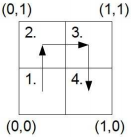
\includegraphics{img/HilbertCurve1-1}
		\caption[labelInTOC]{Hilbert görbe 1. iterációja}
	\end{center}
\end{figure}
\begin{figure}[!ht]
	\begin{center}
		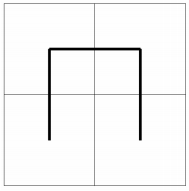
\includegraphics[width=0.5\textwidth]{img/HilbertCurve1-2}
		\caption[labelInTOC]{Hilbert görbe 1. iterációja}
	\end{center}
\end{figure}
A Hilbert-görbe második iterációja 4 egységnégyzetből áll, mindegyikben megrajzolva az első iteráció fordított U alakzatát. A bal alsó négyzetet 90 fokkal jobbra, a jobb alsó négyzetet 90 fokkal balra forgatjuk, így a két alsó U alakzat egymástól "elfelé" néz. Végül az U alakzat megrajzolásával megegyező sorrendben (bal alsó, bal felső, jobb felső, jobb alsó) összekötjük mind a 4 egységnégyzetben levő alakzatok egymáshoz legközelebbre eső végpontjait.
\begin{figure}[!ht]
	\begin{center}
	
\includegraphics[width=0.5\textwidth]{img/HilbertCurve2-1}
	\caption[labelInTOC]{Hilbert görbe 2. iterációja}
\end{center}
\end{figure}


\subsection*{Implementáció}
Az implementáció megvalósításához elengedhetetlen két képlet használata, ezek a következők:\\
$N = 2^I$,
$P = N^2$, ahol N a négyzetek száma, I az iteráció, P pedig a pontok száma. Az iteráció adott, ugyanis a felhasználó konfigurációs lehetőségként meg kell adja, hogy hanyadik iterációig szeretné, hogy az algoritmus fusson. 
Az algoritmus egy setup fügvénnyel indul, ez különbözik a p5.js setup függvényétől, és az alábbi módon néz ki:
\begin{lstlisting}[language=typescript]
 setup(): void {
	 this.squares = Math.pow(2, this.order);
	 this.points = Math.pow(this.squares, 2);
	 this.length = Math.min(this.width, this.height) / this.squares;
	 for (let i = 0; i < this.points; i++) {
		 this.path[i] = this.hilbert(i);
		 this.path[i].mult(this.length);
		 this.path[i].add(this.length / 2, this.length / 2);
	 }
	 this.root = new Line(new p5.Vector(this.path[0].x, this.path[0].y),
	 new p5.Vector(this.path[1].x, this.path[1].y));
 }
\end{lstlisting}
A függvény először, a fentebb említett képletek segítségével kiszámolja, hogy az adott iteráció esetén hány négyzetből, és hány pontból fog állni a Hilbert-görbe. Ezután kiszámolja, hogy mekkora lesz egy-egy vonal hossza. Mivel a vászon szélessége és hosszúsága különbözik, ezért a függvény a kettő közül a kisebbiket veszi számításba, így a görbe biztosan bele fog férni a vászonba, majd ezt leosztja a négyzetek számával. Egy for ciklus segítségével a függvény 0-tól a pontok számáig iterál, és minden iterációban meghívja a hilbert függvényt, amelynek paraméterül a ciklusváltozót adja. A hilbert függvény egy vektort ad vissza, amely megmondja, hogy az adott index, amit paraméterként átadtunk neki, az U alakzat mely pontjával egyezik meg. Ez (0, 0) vektor esetén az alakzat bal felső pontja, (0, 1) esetén a bal alsó pontja, és így tovább... Ezeket a vektorokat egy path nevezetű tömbhöz adja, megszorozza a fentebb kiszámított hosszúsággal, hogy a vektorok közötti távolság megfelelő legyen, majd a vektor x és y értékeihez hozzáadja a hosszúság felét, ezzel megfelelő helyre pozícionálva őket.
\par Az algoritmus draw függvénye a setup függvény által feltöltött path tömbön iterál végig úgy, hogy minden képrfissítéskor eggyel mélyebbre megy a pontok tömbjén, és egy vonallal összeköti az adott pontot a tömbben levő előző ponttal, ezzel egy animációs hatást keltve. 
\par Az algoritmus viszonylag kevés konfigurációs lehetőséggel bír, ezek a következők:
\begin{itemize}
	\item Gyorsaság
	\item Vonalvastagság
	\item Iteráció
	\item Szín
	\item Szivárvány mód
\end{itemize}
\section*{Pitagorasz-fa}
A Pitagorasz-fa egy négyzetekből álló fraktál, amelyet Albert Bosman fedezett fel. A nevét onnan kapta, hogy minden egymást érintő négyzet hármas egy szabályos háromszöget zár be. Ha a legnagyobb négyzet $L x L$ méretű (törzs), akkor a teljes Pitagorasz-fa elfér egy $6L x 4L$ méretű négyzetben. A hagyományos, egyenlő szárú Pitagorasz-fa a következőképpen konstruálható: az első iterációban létrejön a törzse, amely egy négyzet. A második iterációban a törzsnek a felső élére egy egyenlő szárú derékszögű háromszög rajzolunk úgy, hogy átfogója a négyzet felső éle, valamint a háromszög két befogójából kiágazik az első két ág, amelyek szintén négyzetek. Ezután minden iterációban ez ismétlődik, azaz minden korábbi négyzet felső élére egy egyenlő szárú derékszögű háromszög nő, és azok befogói új négyzetágakat növesztenek. Minden négyzet mérete $sqrt(2)/2$ értékkel skálázódik le a szülő négyzet méretéhez képest.
\begin{figure}[!ht]
	\begin{center}
		
\includegraphics[width=0.5\textwidth]{img/PythagorasTree}
		\caption[labelInTOC]{Pitagorasz-fa}
	\end{center}
\end{figure}

\subsection*{Implementáció}
Az kód átláthatósága érdekében itt is egy segédosztályt írtam először. Ebben az osztályban tárolódnak a négyzetek pontjai illetve mérete. Továbbá, két fontos függvényt tartalmaz, az expandLeft és expandRight függvényeket, amelyek az adott négyzet bal és jobb oldali négyzetágait adják meg. 
\begin{lstlisting}[language=typescript]
expandRight(p: any, angle: number): Rectangle {
	let A: p5.Vector;
	let B: p5.Vector;
	let C: p5.Vector;
	let D: p5.Vector = this.B;
	
	let center = p5.Vector.lerp(this.A, this.B, .5);
	let dir = p5.Vector.sub(this.A, center);
	dir.rotate(angle);
	let offset = p5.Vector.add(center, dir);
	
	C = p5.Vector.lerp(center, offset, this.size * 0.5 / p5.Vector.dist(offset, center));
	
	A = p5.Vector.sub(D, C);
	A.rotate(-p.PI/2);
	A = p5.Vector.add(C, A);
	A = p5.Vector.lerp(C, A, 1);
	
	B = p5.Vector.sub(C, D);
	B.rotate(p.PI/2);
	B = p5.Vector.add(D, B);
	B = p5.Vector.lerp(D, B, 1);
	
	let left = new Rectangle(A, B, C, D);
	
	return left;
}
\end{lstlisting}
Az új négyzetek pontjai vektorműveletek sorozatával számolódnak ki. A pontok elnevezése a következő rendszert követi: 
\begin{itemize}
	\item A - bal felső
	\item B - jobb felső
	\item C - bal alsó
	\item D - jobb alsó
\end{itemize}
A jobb oldali négyzetág D pontja megegyezik a szülő négyzet B pontjával. A C pontot úgy kapom meg, hogy a szülő négyzet B pontjából egy vektort hozok létre, amelyből kivonom a szülő négyzet felső élének középpontjából létrehozott vektort, így egy megfelelő irányba mutató vektort kapok, amelyet rotálok egy bizonyos értékkel. A rotálási szöget a függvény paraméterként kapja, ugyanis ez az érték testreszabható a konfigurációs panelben. A maradék A és B pontok már könnyen kiszámolhatóak, ezeket úgy kapom meg, hogy két új vektort hozok létre, egyik a C-ből D-be, másik a D-ből C-be mutat, majd ezeket 90 fokkal rotálom a megfelelő irányba. A függvény visszatérési értékként egy új négyzet objektumot hoz létre a kiszámított pontokból. Az expandLeft függvény hasonlóan működik, csupán a rotálási irányok változnak. 
\par Az algoritmus konfigurációs lehetőségei a következők:
\begin{itemize}
	\item Gyorsaság
	\item Fixált szög
	\item Fixált gyökér
	\item Oldalhosszúság
	\item Szín
	\item Szivárvány mód
\end{itemize}
Ha a fixált gyökér lehetőséget kikapcsoljuk, akkor tetszőleges helyen helyezhetünk el gyökér négyzetet a vászonon, ezt az egér görgője segítségével rotálhatjuk, illetve az oldalhosszúság opció érékének változtatásával megadhatjuk a méretét. Hasonlóan, a fixált szög lehetőség kikapcsolásával tetszőleges szöggel elhajlíthatjuk a négyzetágakat jobb vagy bal irányba. A szög megadása az egér segítségével történik. Ahhoz, hogy a felhasználóknak érthető legyen a szög megadásának módja, a törzs négyzet felső élének középpontjából egy egyenes indul az egérmutató pozíciója felé. Ennek egyenesnek a hossza az oldalhosszúság felével egyezik meg. Kattintáskor a program kiszámolja az egyenes és a négyzet felső éle között bezárt szöget, és ezt felhasználja a négyzetágak generálásakor.
\section*{Fraktál-fa}
A Fraktál-fa egy viszonylag egyszerűen megkonstruálható fraktál, ami a legismertebb fraktálok közé tartozik. Szerkezete nagyon hasonlít a Pitagorasz-fához, annyi különbséggel, hogy négyzetek helyett egyszerű vonalakból tevődik össze. A Fraktál-fa első iterációjában csak a törzs van, a másodikban a törzsből két ág nő ki egy bizonyos szöget bezárva a törzzsel. Ez a szög tetszőlegesen állítható a konfigurációs panelben. A további iterációkban ez ismétlődik, tehát a már meglévő ágakből új ágak nőnek ki, ez a végtelenségig ismételhető.  
\begin{figure}[!ht]
	\begin{center}
		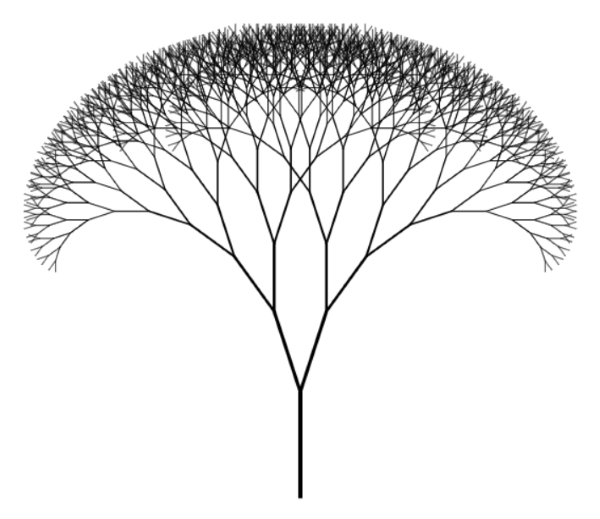
\includegraphics[width=0.5\textwidth]{img/FractalTree}
		\caption[labelInTOC]{Fraktál fa}
	\end{center}
\end{figure}
\subsection*{Implementáció}
A szerkezeti hasonlóságokból eredően az algoritmus implementációja sok helyen hasonlít a Pitagorasz-fáéhoz. Itt is egy segédosztály megírásával kezdtem az implementációt. Ez az osztály tárolja a vonalak A és B végpontjait, valamint hosszát, ezen kívül még tartalmaz egy branch nevezetű függvényt, amely egy adott vonalra meghívva kiszámolja annak az ágait. 
\begin{lstlisting}
branch(p: any, angleLeft: number, angleRight: number, lerpPercentage: number): Line[] {
	let lines: Line[] = [];
	let lerpAmount = this.length * lerpPercentage / this.length;
	
	let dir = p5.Vector.sub(this.A, this.B);
	let xRotated = dir.rotate(angleLeft);
	let xOffset = p5.Vector.add(this.A, xRotated);
	let yRotated = dir.rotate(-angleLeft - angleRight);
	let yOffset = p5.Vector.add(this.A, yRotated);
	let x = p5.Vector.lerp(this.A, xOffset, lerpAmount);
	let y = p5.Vector.lerp(this.A, yOffset, lerpAmount);
	
	lines.push(new Line(x, this.A));
	lines.push(new Line(y, this.A));
	
	return lines;
}
\end{lstlisting}
Ennek a függvénynek 3 fontos paramétere van, az angleLeft, ami megadja a bal oldali ág és a szülő ág által bezárt szöget, az angleRight, ami a jobb oldali ág és a szülő ág által bezárt szöget adja meg, valamint a lerpPercentage, ami azt adja meg, hogy az ágak hossza hány százaléka a szülő ág hosszának. Mivel az egyes vonalak A és B végpontjait vektor típusokként tárolja a segédosztály, ezért az új ágak végpontjai vektorműveletek segítségével könnyen kiszámolhatóak. Az A végpontból kivonva a B végpontot, egy, a vonal irányával megegyező irányú vektort kapok. Ezt, a paraméterben kapott értékekkel jobbra és balra forgatva, megkapom az új ágak A végpontjait. Az új ágak B végpontjai a szülő ág A végpontjával egyeznek meg értelemszerűen. A visszatérési értéke egy tömb, amely az új ágakat tartalmazza.
\par Az algoritmus konfigurációs lehetőségei a következők:
\begin{itemize}
	\item Gyorsaság
	\item Vonalvastagság
	\item Vonalhosszúság
	\item Ágak száma
	\item Elforgatási szög
	\item Ág mérete (\%)
	\item Véletlenszerű szög
	\item Fixált kezdővonal
	\item Szín
	\item Szivárvány mód
\end{itemize}
Az ágak száma opcióval megadható, hogy az egyes ágakból 2 vagy 3 új ág keletkezzen, 3 ág esetén a középső ág iránya megegyezik a szülő ág irányával. A fixált kezdővonal opció kikapcsolásával a fa törzsét adhatjuk meg tetszőlegesen, hasonlóan, mint az előző algoritmusoknál.
\section*{H-fa}
A H-fa struktúrája hasonló a Fraktál-fáéhoz. Ez a fraktál merőleges vonalak közvetlen egymás mellé helyezésével konstruálható meg. Minden vonal mindkét végpontján egy rá merőleges vonal halad át, amelynek hossza mindig $sqrt(2)$-vel kisebb az előző vonal hosszától. Ez egy alapértelmezett érték, ami a konfigurációs panelben tetszőlegesen állítható. A fraktál a nevét onnan kapta, hogy a benne ismétlődő minta a H betűre emlékeztet.\\ 
A H-fa Hausdorff dimenziója 2.
\begin{figure}[!ht]
	\begin{center}
		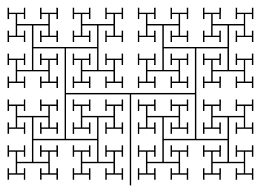
\includegraphics[width=0.5\textwidth]{img/HTree}
		\caption[labelInTOC]{H-fa}
	\end{center}
\end{figure}
\subsection*{Implementáció}
A H-fa egy viszonlyag egyszerűnek mondható fraktál, ezért az implementációja is egyszerű. A függvények, amelyek az ágak pontjainak kiszámolását végzik itt is egy segédosztályban vannak megírva, ezek az expandLeft és expandRight függvények.
\begin{lstlisting}
expandLeft(p: any, lerp: number) {
	let dir = p5.Vector.sub(this.A, this.B);
	dir.rotate(p.PI / 2);
	let xOffset = p5.Vector.add(this.A, dir)
	let x = p5.Vector.lerp(this.A, xOffset, lerp / 2);
	
	dir.rotate(-p.PI);
	let yOffset = p5.Vector.add(this.A, dir);
	let y = p5.Vector.lerp(this.A, yOffset, lerp / 2);
	
	return new Line(x, y);
}
\end{lstlisting}
A segédosztályban a vonalak végpontjai itt is vektorokként vannak tárolva. A végpontokat egymásból kivonva egy vektort kapunk, amelynek iránya megegyezik a vonal irányával, majd ezt jobbra és balra forgatva megkapjuk az bal oldali ág két végpontját. A két új végpontot nem teljesen kötjük össze a szülő vonal bal oldali végpontjával, az új végpontok irányába csak az új ág hosszának a felével megegyező mértékig megyünk, ezzel megkapva az ág megfelelő hosszát. A jobb oldali ág kiszámítása hasonlóan történik.
\par Az algoritmushoz tartozó konfigurációs lehetőségek a következők:
\begin{itemize}
	\item Gyorsaság
	\item Vonalvastagság
	\item Vonalhosszúság
	\item Ág hosszúság (\%)
	\item Fixált kezdővonal
	\item Szín
	\item Szivárvány mód
\end{itemize}
\chapter*{Összegzés}
\addcontentsline{toc}{section}{Összegzés}
\spacing{1.5}
Szakdolgozatom többnyire a fraktál bemutató keretrendszer implementálásának menetét mutatta be. Ez egy olyan keretrendszer amely a felhasználóknak lehetőséget ad arra, hogy nyolc féle fraktált generáljanak, a generáló algoritmusokat konfigurálják, az eredményt képként exportálják, a generálás közben visszalépjenek valamely előző lépésre, valamint mind a nyolc keretrendszerben szereplő fraktálról egy rövid bemutatót olvassanak.
\par A szakdolgozat elején az olvasók a fraktálokról egy bemutatót olvashatnak. Szó van a fraktálok tulajdonságairól, alkalmazási területeiről, nevének eredetéről. Ez a fejezet lényegében a fraktálok mivoltáról szól. A fraktálok röviden fogalmazva olyan alakzatok, amelyek szerkezetében legalább egy felismerhető ismétlődés található. A fraktálok legfontosabb tulajdonsága az önhasonlóság.
\par Az ezt követő szekcióban az interneten található hasonló webalkalmazásokról van szó röviden, ismertetem a felhasznált technológiákat, amelyek az Angular keretrendszer, és a p5.js, ami egy vászon rajzolásra alkalmas JavaScript könyvtár. 
\par A további fejezetek témáját maga a keretrendszer tölti ki. Bemutatásra kerülnek az alkalmazás főbb funkciói, amelyek többek között a konfigurálás, exportálás, és visszatekerés. Részletezem mindegyik fraktál generáló algoritmus implementációjának menetét, valamint az alkalmazásban szereplő minden fraktálról egy ismertetőt olvashatnak. A keretrendszer részeként implementált nyolc fraktál generáló algoritmus a következő: 
\begin{itemize}
	\item Sierpiński- háromszög
	\item Sierpiński-szőnyeg
	\item Fraktál-fa
	\item Pitagorasz-fa
	\item Lévy C-görbe
	\item Koch-görbe
	\item Hilbert-görbe
	\item H-fa
\end{itemize}
\par Az elkészült alkalmazást a jövőben bővíteni szeretném. A már megírt algoritmusokhoz további konfigurációs lehetőségeket tervezek implementálni, valamint a magát keretrendszert kibővíteni még néhány fraktál algoritmussal, mint például a Sárkány-görbe, vagy a Sam-görbe.


%Irodalomjegyzek ha kell
\bibliography{mybib}
\bibliographystyle{plain}

\chapter*{Nyilatkozat}
%Egy üres sort adunk a tartalomjegyzékhez:
\addtocontents{toc}{\ }
\addcontentsline{toc}{section}{Nyilatkozat}
%\hspace{\parindent}

% A nyilatkozat szövege más titkos és nem titkos dolgozatok esetében.
% Csak az egyik tipusú myilatokzatnak kell a dolgozatban szerepelni
% A ponok helyére az adatok értelemszerûen behelyettesídendõk es
% a szakdolgozat /diplomamunka szo megfeleloen kivalasztando.


%A nyilatkozat szövege TITKOSNAK NEM MINÕSÍTETT dolgozatban a következõ:
%A pontokkal jelölt szövegrészek értelemszerûen a szövegszerkesztõben és
%nem kézzel helyettesítendõk:

\noindent
Alulírott \makebox[4cm]{\dotfill} szakos hallgató, kijelentem, hogy a dolgozatomat a Szegedi Tudományegyetem, Informatikai Intézet \makebox[4cm]{\dotfill} Tanszékén készítettem, \makebox[4cm]{\dotfill} diploma megszerzése érdekében.

Kijelentem, hogy a dolgozatot más szakon korábban nem védtem meg, saját munkám eredménye, és csak a hivatkozott forrásokat (szakirodalom, eszközök, stb.) használtam fel.

Tudomásul veszem, hogy szakdolgozatomat / diplomamunkámat a Szegedi Tudományegyetem Informatikai Intézet könyvtárában, a helyben olvasható könyvek között helyezik el.

\vspace*{4cm}

\begin{tabular}{lc}
Szeged, \today\
\hspace{2cm} & \makebox[6cm]{\dotfill} \\
& aláírás \\
\end{tabular}


\vspace*{2cm}

%A nyilatkozat szövege TITKOSNAK MINÕSÍTETT dolgozatban a következõ:

%\noindent
%Alulírott \makebox[4cm]{\dotfill} szakos hallgató, kijelentem, hogy a dolgozatomat a Szegedi Tudományegyetem, Informatikai Intézet \makebox[4cm]{\dotfill} Tanszékén készítettem, \makebox[4cm]{\dotfill} diploma megszerzése érdekében.

%Kijelentem, hogy a dolgozatot más szakon korábban nem védtem meg, saját munkám eredménye, és csak a hivatkozott forrásokat (szakirodalom, eszközök, stb.) használtam fel.

%Tudomásul veszem, hogy szakdolgozatomat / diplomamunkámat a TVSZ 4. sz. mellékletében leírtak szerint kezelik.

%\vspace*{1cm}

%\begin{tabular}{lc}
%Szeged, \today\
%\hspace{2cm} & \makebox[6cm]{\dotfill} \\
%& aláírás \\
%\end{tabular}

\chapter*{Köszönetnyilvánítás}
\addcontentsline{toc}{section}{Köszönetnyilvánítás}
Köszönöm a figyelmet.




\end{document}